HARCAD is a system to
explore ``Cyborg Craft'', a new kind of undigital craft: being undigital
with digital computers.
One such embodiment is the T-SWIM
(Fig~\ref{fig:tswim})
as a haptic augmented reality interaction device and system.
In this system, one or more users can grasp and touch and feel virtual
objects in cyborgspace, and share the resulting haptic augmented reality
experience, as a way of designing and making things like cars,
buildings, furniture, etc., through a collaborative design and
realization process.

Let's consider a simple example.  We wish to make a table with a nice
curvy shape to it.  A good place to begin is with waves.
As a basis for synthesis, we have a shape synthesizer.
In some embodiments the shape synthesizer is made in software,
from simple shapes like rectangles, circles, ellipses, etc., as one
might find in a computer program like Interviews idraw,
Inkscape, or Autodesk Fusion 360.
In other embodiments the shape synthesizer exists as a piece of hardware,
as illusrated in Fig~\ref{fig:wavetable}.
\begin{figure}
  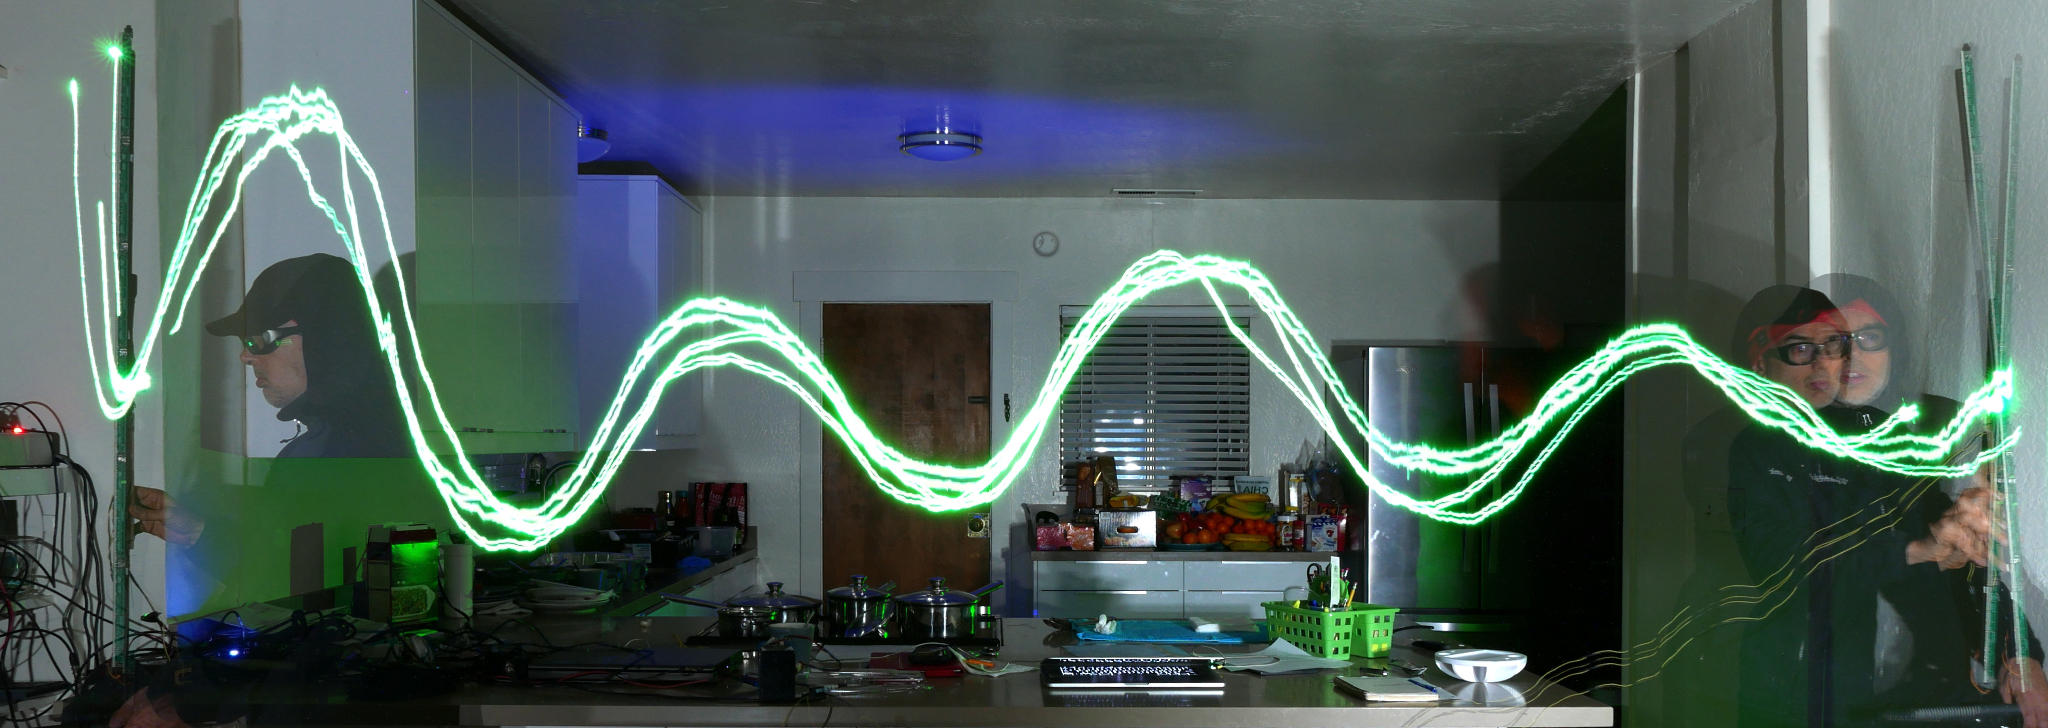
\includegraphics[width=\linewidth]{threefundamentals_and_me_dccq.jpg}
  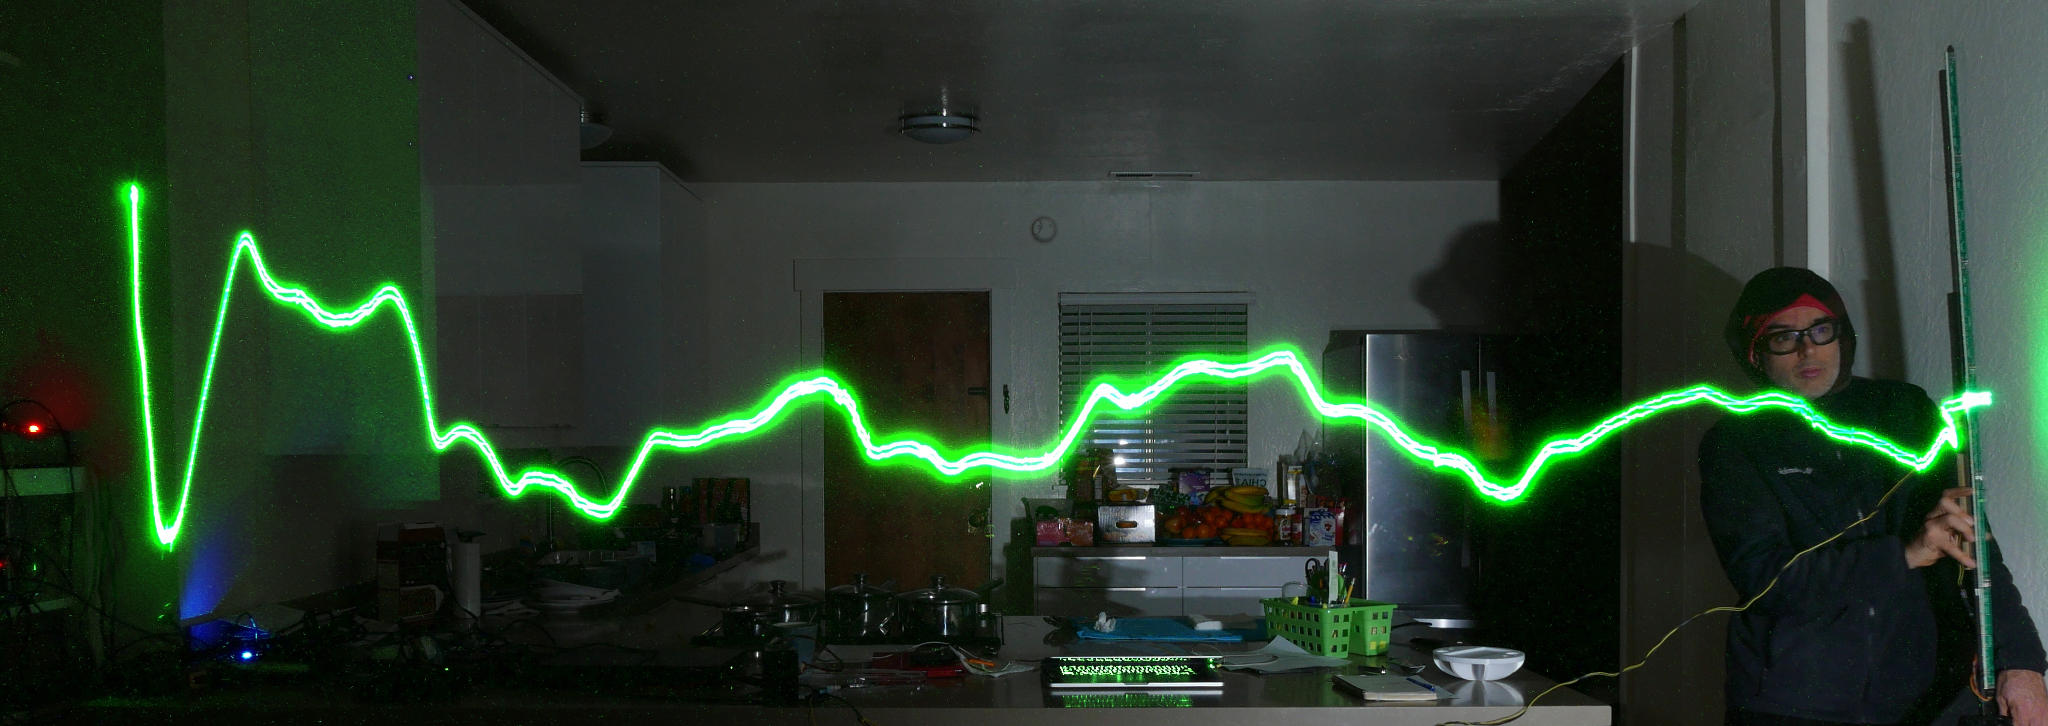
\includegraphics[width=\linewidth]{wave87_and_me90_dccq.jpg}
  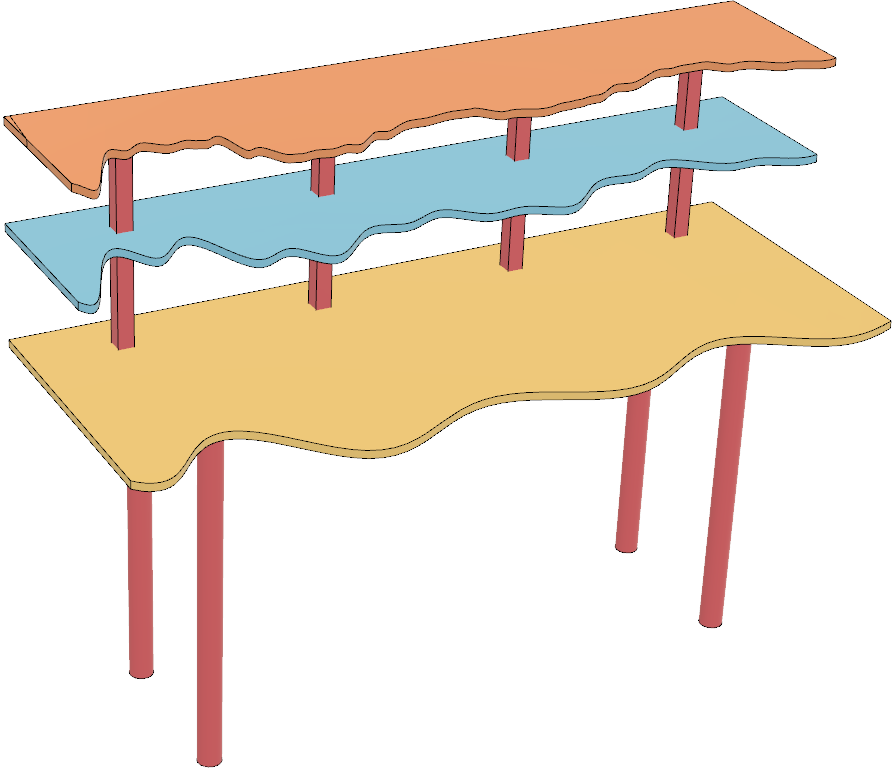
\includegraphics[width=\linewidth]{WaveTableFusion360.png}
  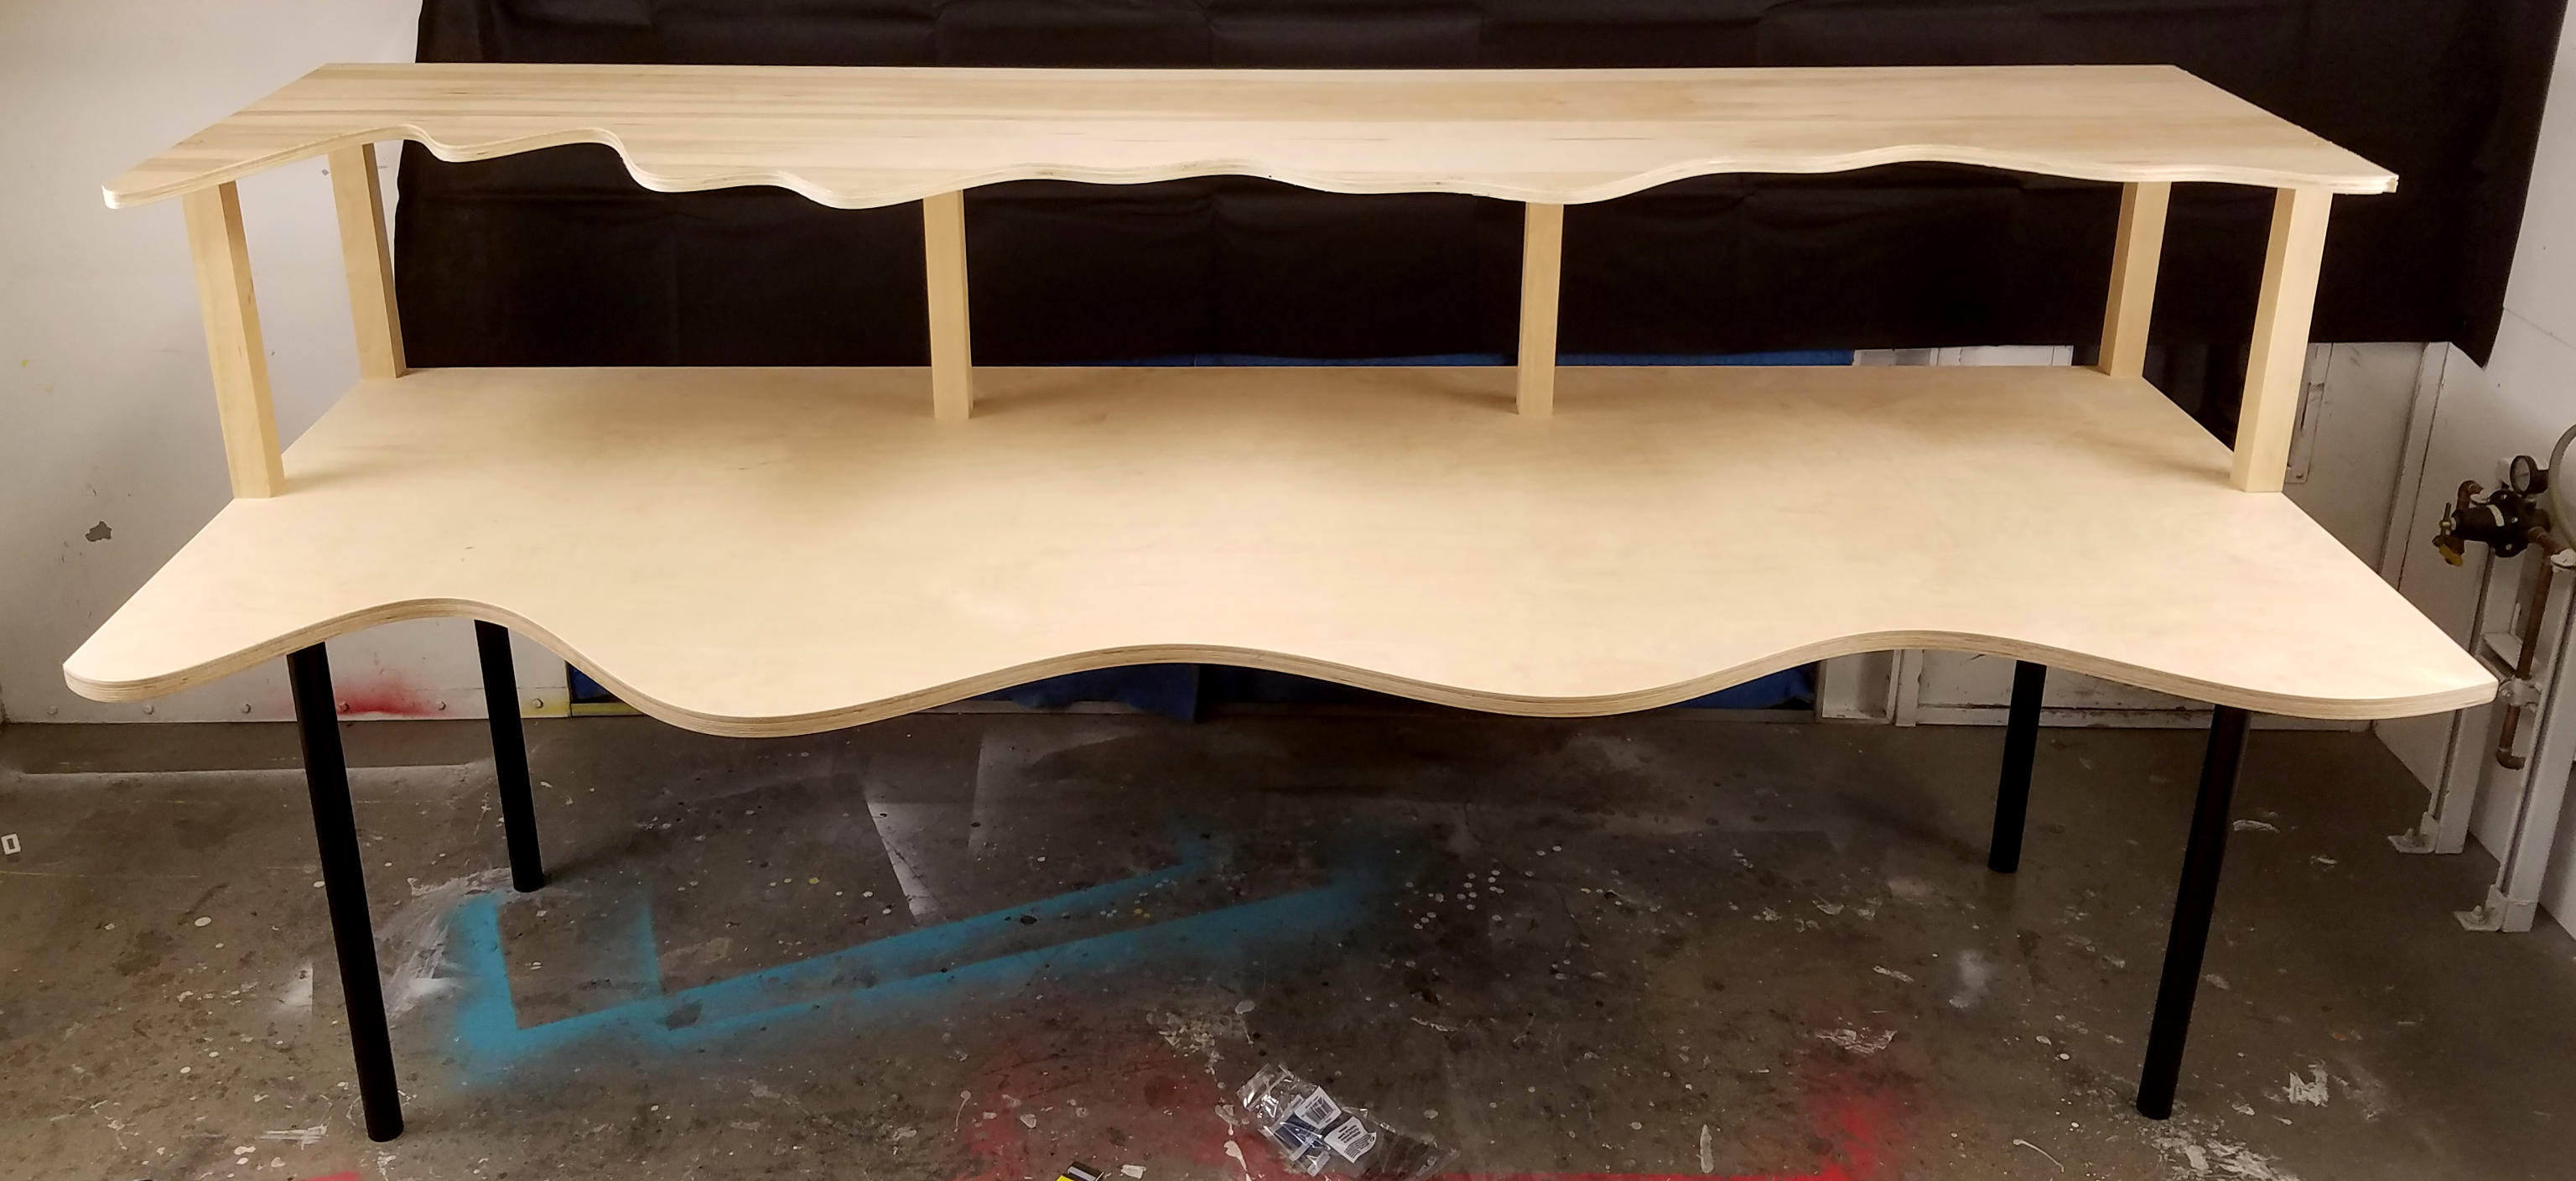
\includegraphics[width=\linewidth]{wavetable_20161129_214045cq.jpg}
  \caption{
           {\bf Furniture design with Haptic Augmented Reality
                CAD/CAM}.
           A shape generator or shape synthesizer, such as
           a PASCO SCIENTIFIC MODEL WA-9307 FOURIER SYNTHESIZER,
           generates shape information which is visualized in alignment
           with haptic sensation, so that shapes can be seen and felt in
           perfect alignment.
           A 3D (3-dimensional) wireless position sensor comprises
           transducers with phase-coherent detection.
           The synthesizer is connected to a fixed transducer (loudspeaker),
           and the reference input of a NARLIA (Natural Augmented Reality
           Lock-In Amplifier).  A moving transducer (microphone) on a
           Haptic Augmented Reality CAD (HARCAD) wand is connected to the
           signal input of the NARLIA.
           An output from the NARLIA is connected to a T-SWIM, here, 600
           LEDs and a vibrotactile actuator, both part of the HARCAD wand.
           As the user moves the wand back-and-forth, a multisensory
           experience results in which the user can see, feel, and
           hear the virtual shapes (e.g. waves and their harmonics).
           Arbitrary shapes can be generated by Fourier synthesis,
           and these shapes can be touched, felt, and manipulated.
          }
  \label{fig:wavetable}
\end{figure}
Here is a multiple exposure, showing three exposures while
moving back-and-forth, which align, approximately, with each other,
while admitting a small variation.
The shape is sculpted by press-pull operations.
Additionally, harmonic variations are made to the shapes, to
design furniture.
Here a wavetable is designed in which the table is the
fundamental of the waveform from a musical note, and the shelf
above it is the fundamental and first overtone
(i.e. the first two harmonics).
Here the amplitude of the waveforms decreases from left-to-right
as we move further from the sound source.

